\section{\review{Coordinate Systems}}

In circular accelerators, particle dynamics are represented using a comoving coordinate system.
A reference orbit is determined by the lattice and its magnet strengths. A set of given strengths 
for a lattice is called \textit{optics}. In the case of a synchrotron, like the LHC, the reference
orbit is also called the closed orbit.

The Frenet-Serret coordinate system moves along the ring on the reference orbit. The coordinates are
then transverse: $x$ and $y$, and longitudinal in the direction of travel: $s$.
\Cref{fig:coordinate_systems:frenet_serret} shows these coordinates.

\begin{figure}[H]
    \centering
    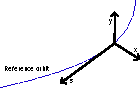
\includegraphics[width=0.5\textwidth]{images/frenet.pdf}
    \caption{Frenet-Serret coordinate system, commonly used in accelerator physics. The system moves
    along the reference orbit.}
    \label{fig:coordinate_systems:frenet_serret}
\end{figure}

This coordinate system is widely used to simply describe either an element's or a particle's
position in the accelerator. Without any explicit mention, these are the coordinates used in this
thesis. It is frequent to use the variable $z$ to refer to either $x$ or $y$ in equations.
In order to describe the motion of particles through a lattice, different coordinate systems can be
used. To better describe the motion of particles through a lattice, various coordinate systems can
be employed. First, the formalism for a linear lattice will be introduced, followed by an
explanation of how motion in a machine with non-linear elements can be characterized.

Linear optics refer to the regime where the forces acting on particles, such as those from dipoles
and quadrupoles, are directly proportional to the particle's displacement from the reference
trajectory, resulting in simple, predictable motion described by linear equations and transfer
matrices. Non-linear optics, on the other hand, involves higher-order magnetic elements like
sextupoles and octupoles, where the forces are non-linear with respect to displacement. This leads
to more complex particle motion, which can result in phase-space distortions and chaotic
trajectories.


% ============================================
%               Linear Lattice 
% ============================================
\subsection{\review{Linear Lattice}}

% ========================
% Courant-Snyder Parameters
\subsubsection{\review{Courant-Snyder Parameters}}
\label{section:courant_snyder}

A circular accelerator is composed of many multipoles of different orders. A very basic
design only requires dipoles and quadrupoles in order to operate. Dipoles are used to bend the
particles to form the ring, whereas quadrupoles are used to focus the beam to a focal
point, similar to photons with lenses.
Those elements can be arranged in a particular order, to form a FoDo cell. Such cells present an
alternating placement of focusing an defocusing quadrupoles with dipoles in between, as shown in
\cref{fig:coordinate_systems:fodo}, and are usually repeated many times along the ring.

\begin{figure}[htb]
    \centering
    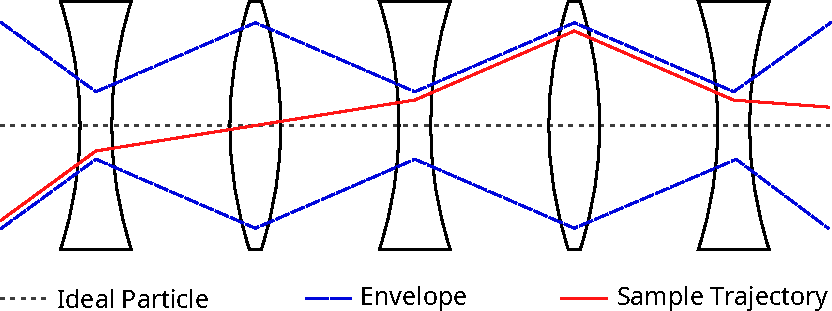
\includegraphics[width=0.8\textwidth]{images/fodo_drawing.pdf}
    \caption{Line composed of FoDo cells, a basic cell present in most accelerators, composed of a
    Focusing and a Defocusing quadrupole. The envelope of the beam is influenced by the
    $\beta$-function and the action $J$.}
    \label{fig:coordinate_systems:fodo}
\end{figure}

A lattice composed of only dipoles and quadrupoles, is referred to as a \textit{linear} lattice. In
a synchrotron, a circular particle accelerator, particles undergo transverse and longitudinal 
oscillations. 
These oscillations usually describe an ellipse in phase-space, a system with position $z$ and
momentum $p_z$ as coordinates.
Taking into account those oscillations, the phase-space ellipse of a particle at a position $s$ in
the ring can be described with a new system: the Courant-Snyder parameters, also know as Twiss
parameters or the \textit{optics functions}~\cite{courant_theory_1958}, as shown in
\cref{fig:coordinate_systems:twiss}.

\begin{figure}[htb]
    \centering
    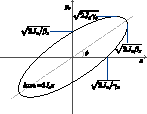
\includegraphics[width=0.6\textwidth]{images/phase_space.pdf}
    \caption{Phase-space ellipse of a linear machine, parametrized by the Courant-Snyder
    parameters $\alpha$, $\beta$ and $\gamma$.}
    \label{fig:coordinate_systems:twiss}
\end{figure}

$J$, the action, is the invariant of linear motion at a given energy and describes the amplitude of
oscillations. It is related to the other quantities by:

\begin{equation}
    J_z = \frac{1}{2} (\gamma_z \cdot z^2 + 2 \alpha_z p_z \cdot z + \beta_z p_z^2).
    \label{eq:coordinate_systems:action}
\end{equation}

The area of the phase-space ellipse is also called the single particle emittance, and is described
by the action: 
$\epsilon = 2J$.  As the $\beta$ parameter varies along the ring, it is referred to as the
$\beta$-function and is related to the amplitude of the oscillations. Thus, the smaller is the
$\beta$-function, the smaller is also the envelope of the beam.
The number of oscillations per turn is called the \textit{tune}, and is closely related to the
$\beta$-function:

\begin{equation}
    Q_{x,y} = \frac{1}{2 \pi} \oint \frac{1}{\beta_{x,y}(s)} \diff s.
    \label{eq:coordinate_systems:tune}
\end{equation}


It is common to express the position of a particle using \textit{action-angle} variables:
% allowing to switch between the Courant-Snyder parameters and the Frenet-Serret system:

\begin{equation}
    \begin{aligned}
    z   &= \sqrt{2J_z \beta_z} \cos{\phi_z} \\
    p_z &= - \sqrt{\frac{2J_z}{\beta_z}} \left( sin{\phi_z} + \alpha_z \cos{\phi_z}\right).
    \end{aligned}
    \label{eq:coordinate_systems:action_angle}
\end{equation}


\subsubsection{\review{Normalized Coordinates}}

In order to simplify the description of the linear motion in a ring, a transformation can be applied
to the previously seen coordinates. \Cref{fig:coordinate_systems:normalized_coordinates}
shows a phase-space described in both coordinates. The new coordinates, $\hat{z}$, and $\hat{p}_z$,
are then expressed as factors of the $\alpha$ and $\beta$ functions:

\begin{equation}
    \begin{pmatrix}
        \hat{z}    \\
        \hat{p}_z 
    \end{pmatrix}
    =
    \begin{pmatrix}
        \frac{1}{\sqrt{\beta_z}}         &   0 \\
        \frac{\alpha_z}{\sqrt{\beta_z}}  &   \sqrt{\beta_z}
    \end{pmatrix}
    \begin{pmatrix}
        z \\
        p_z 
    \end{pmatrix}.
\end{equation}

This allows to describe the motion as a simple rotation, the new coordinates being only dependent on
the invariant $J_z$ and the phase $\phi_z$:

\begin{equation}
    \begin{aligned}
        \hat{z}   &= \sqrt{2J_z} \cos \left(\phi_z \right), \\
        \hat{p}_z &= \sqrt{2J_z} \sin \left(\phi_z \right).
    \end{aligned}
\end{equation}     

\begin{figure}[H]
    \centering
    \begin{subfigure}[b]{0.4\textwidth}
        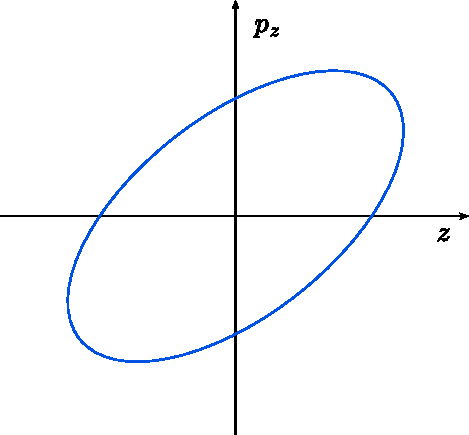
\includegraphics[width=\linewidth]{images/phase_space_regular_coordinates.pdf}
        %\caption{Caption for Image 1}
        %\label{fig:sub1}
    \end{subfigure}
    \begin{subfigure}[b]{0.4\textwidth}
        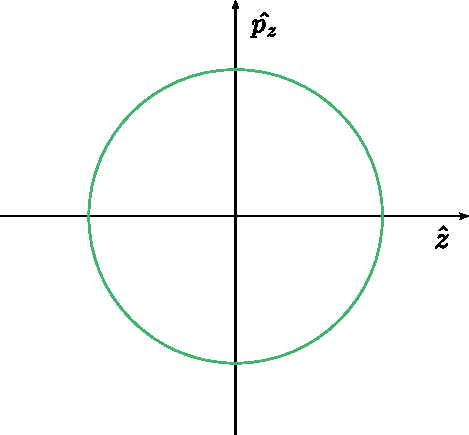
\includegraphics[width=\linewidth]{images/phase_space_normalized_coordinates.pdf}
        %\caption{Caption for Image 2}
        %\label{fig:sub2}
    \end{subfigure}
    \caption{Phase space described in both regular and normalized coordinates.}
    \label{fig:coordinate_systems:normalized_coordinates}
\end{figure}


% ========================
% Linear Transfer Map
\subsubsection{\review{Linear Transfer Maps}}
\label{section:coordinate_systems:linear_maps}

The final position of a particle after passing through an accelerator element can be described using
\textit{transfer maps}. In the case of linear optics, these maps take the form of matrices.
Importantly, these maps should be symplectic, meaning the area of the phase-space ellipse is
preserved, ensuring that the particle's motion is accurately represented. Symplecticity guarantees
that key properties of the beam, such as its emittance, remain constant, which is crucial for
maintaining the stability and integrity of particle trajectories in tracking simulations.
For a matrix $M$ and positions $z$ at the initial location and at $s$, the general formula
reads~\cite{lee_accelerator_2004}:

\begin{equation}
    \begin{pmatrix}
        z \\
        z'
    \end{pmatrix}_s
    = M \cdot 
    \begin{pmatrix}
        z \\
        z'
    \end{pmatrix}_0
\end{equation}

This formalism assumes that the magnetic field is linear or constant along the element in the
longitudinal direction. Basic elements such as drifts, dipoles, quadrupoles can then be described be
a simple $2 \times 2$ matrix:

\begin{equation}
    M_{drift} = \begin{pmatrix}
                    1 & L \\
                    0 & 1 
                \end{pmatrix},
\end{equation}
\begin{equation}
    M_{dipole} = \begin{pmatrix}
                    \cos\left(L/\rho\right) & \rho \sin\left(L/\rho\right) \\
                    -1/\rho \sin\left(L/\rho\right) & \cos\left(L/\rho\right)
                 \end{pmatrix}, \\
\end{equation}
\begin{equation}
    M_{focusing\;quad.} = \begin{pmatrix}
                             \cos\left(\sqrt{k_2}L\right) & 1/\sqrt{k_2} \sin\left(\sqrt{k_2}L\right) \\
                             -\sqrt{k_2}\sin\left(\sqrt{k_2}L\right) & \cos\left(\sqrt{k_2}L\right)
                          \end{pmatrix},\\
\end{equation}
\begin{equation}
    M_{defocusing\;quad.} = \begin{pmatrix}
                        cosh\left(\sqrt{|k_2|}L \right) & 1/\sqrt{|k_2|} sinh\left(\sqrt{|k_2|} L\right) \\
                        \sqrt{|k_2|} sinh\left(\sqrt{|k_2|} L\right) & cosh\left(\sqrt{|k_2|} L \right)
                            \end{pmatrix},\\
\end{equation}

where L is the length of the element, $\rho$ the radius of curvature of the orbit and $k_2$ the
normalized strength of quadrupoles. In the case of quadrupoles, a focusing matrix should be used in
the horizontal plane for focusing quadrupoles, where defocusing matrices should be used in the
vertical plane. The opposite goes for defocusing quadrupoles.

Transfer matrices can be combined together to describe a larger group of elements, as the FoDo cell
seen previously. Its transfer matrix can then be expressed as,

\begin{equation}
    M_{FoDo} = M_{focusing\;quad} \cdot M_{drift} \cdot M_{defocusing\;quad} \cdot M_{drift}.
\end{equation}

For a closed machine, a full revolution can be described by a so-called \textit{one-turn map}, being
the transfer matrix of the whole machine, denoted $\mathcal{M}$. Such a map can potentially contain
thousands of elements.


% ============================================
%             Non-Linear Lattice 
% ============================================
\subsection{\review{Non-Linear Lattice}}

So far, Courant-Snyder parameters were a good way to describe the distribution of positions and
velocities of particles in the transverse plane. One caveat of using this formalism is that it is 
restrained to linear optics and does not address non-linear elements, like octupoles. These elements
generate forces that are not directly proportional to a particle's displacement from the reference
trajectory.
Effects such as resonances or those arising from an arrangement of several multipoles together can
be described by the concepts introduced in this section.
An overview of the needed mathematical tools is first given, before introducing maps.

% ========================
% Lie Algebra
\subsubsection{\review{Lie Algebra}}

One way to describe non-linear effects is to introduce Lie Algebra~\cite{dragt_overview_2013}, a
powerful algebra able to describe transformations, symmetries and their associated conserved
quantities. 
The Lie algebra is a vector space, denoted $\mathfrak{g}$, equipped with a binary operation called
the \textit{Lie bracket} and denoted $[x, y]$ for two vectors $x$ and $y$. Any vector space equipped
with a Lie bracket (or commutator) satisfying the following conditions is called a Lie
algebra:

\begin{itemize}
    \item Bilinearity:
    \begin{equation}
        \begin{aligned}
        \relax[ax+by, z] &= a[x,z] + b[y,z], \\
        [z, ax+by] &= a[z,x] + b[z,y], \quad \forall x,y,z \in \mathfrak{g}~\text{and}~a,b~\text{scalars}
        \label{eq:coordinates:bilinearity}
        \end{aligned}
    \end{equation}

    \item Alternativity:
    \begin{equation}
        [x,x] = 0, \quad \forall x \in \mathfrak{g}
    \end{equation}

    \item Anticommutativity:
    \begin{equation}
        [x,y] = -[y,x], \quad \forall x,y \in \mathfrak{g}
    \end{equation}

    \item The Jacobi identity:
    \begin{equation}
        [x,[y,z]] + [y, [z,x]] + [z, [x,y]] = 0, \quad \forall x,y,z \in \mathfrak{g}
        \label{eq:coordinates:jacobi_identity}
    \end{equation}
\end{itemize}

The \textit{Lie bracket}, plays a central role in the Lie algebra. It describes how dynamical
variables evolve under infinitesimal symplectic transformations.


% ========================
% Poisson Brackets
\subsubsection{\review{Poisson Brackets}}

In accelerator physics, following the Hamiltonian formalism and classical mechanics, the commutator
is represented by the \textit{Poisson brackets}, which satisfy the necessary conditions for
describing particle motion~\cite{dragt_overview_2013,roy_analysis_1992}. Poisson brackets are used
to express continuous symmetries, conserved quantities, and the time evolution of dynamical
variables within the system. 

Let's consider position and momentum coordinates $q_i \cdots q_n$ and $p_i \cdots p_n$  of a
2n-dimensional phase space. Usually, those would be $x, y, p_x \text{ and } p_y$ for transverse
coordinates. The Poisson brackets of two functions $f$ and $g$ is then defined by:

\begin{equation}
    [f,g] = \sum^n_{i=1} \frac{\partial f}{\partial q_i} \frac{\partial g}{\partial p_i}
                       - \frac{\partial f}{\partial p_i} \frac{\partial g}{\partial q_i}.
    \label{eq:coordinate_systems:poisson_bracket}
\end{equation}


The evolution of coordinates and momenta in time is described by Hamilton's equations of motion, which can
be naturally expressed with Poisson brackets:

\begin{equation}
    \begin{aligned}
        \frac{\partial H}{\partial p_i}   &= \frac{\diff q_i}{\diff t}  &&= [q_i, H] \\
       -\frac{\partial H}{\partial q_i}   &= \frac{\diff p_i}{\diff t}  &&= [p_i, H].
    \end{aligned}
\end{equation}


% ========================
% Lie Operator
\subsubsection{\review{Lie Operator}}

Given a function $f$, a differential operator called \textit{Lie operator} is defined, and is closely
related to the previously seen Poisson bracket:

\begin{equation}
:f: = \sum^n_{i=1} \frac{\partial f}{\partial q_i} \frac{\partial}{\partial p_i}
                    - \frac{\partial f}{\partial p_i} \frac{\partial}{\partial q_i}.
\end{equation}

The action of this operator on a function $g$ is equivalent to the Poisson brackets, as in:

\begin{equation}
    :f:g = [f,g].
\end{equation}

A particular power series of this Lie operator can now be defined, called \textit{Lie
transformation}:

\begin{equation}
    \begin{aligned}
        e^{:f:}g &= \sum_{l=0}^\infty \frac{1}{l!} :f:^l g \\
                 &= g + [f,g] + \frac{1}{2!}[f, [f, g]] + \cdots .
    \end{aligned}
    \label{eq:coordinate_systems:expansion_exponential}
\end{equation}



% ========================
% Non-Linear Transfer Map
\subsubsection{\review{Non-Linear Transfer Maps}}

As introduced in \cref{section:coordinate_systems:linear_maps}, the dynamics of a particle beam in a
circular accelerator can be described by \textit{transfer maps}. A symplectic \textit{One Turn Map}
$\mathcal{M}$ that includes $N$ non-linear elements is defined~\cite{dragt_overview_2013} as,

\begin{equation}
    \mathcal{M} = e^{:h_N:} \cdot e^{:h_{N-1}:} \cdots e^{:h_1:} \cdot \mathcal{R}
\end{equation}

where $\mathcal{R}$ is a matrix describing the linear motion over one turn and the $h_i$ terms
representing the Hamiltonian of each non-linear elements of the machine.
Via the Baker-Campbell-Hausdorff (BCH) theorem~\cite{forest_beam_1998,casas_efficient_2009},
previous Lie transformations can be combined and simplified via
\cref{eq:coordinates:basic_exponent_bch} and \cref{eq:coordinates:bch}. Further orders can be found
and computed via~\cite{casas_efficient_2009}.

\begin{equation}
    e^{:h_1:} \cdot e^{:h_2:} = e^{:h:}
    \label{eq:coordinates:basic_exponent_bch}
\end{equation}
with 
\begin{equation}
    \begin{alignedat}{3}
      h =& h_1 + h_2  && \Rightarrow \text{1\textsuperscript{st} order}\\
             & + \frac{1}{2} [h_1, h_2]  && \Rightarrow \text{2 \textsuperscript{nd} order}\\
             & + \frac{1}{12} [h_1, [h_1, h_2]] - \frac{1}{12} [h_2, [h_1, h_2]] \quad && \Rightarrow \text{3\textsuperscript{rd} order}\\
             & + \cdots.
    \end{alignedat}
    \label{eq:coordinates:bch}
\end{equation}


The one turn map is thus expressed as a single Lie transformation:

\begin{equation}
    \mathcal{M} = e^{:h:} \cdot \mathcal{R}.
   \label{eq:coordinate_systems:non_linear_map}
\end{equation}

In most cases, where the non-linear perturbations are small, the above series converges quickly
and only the first order of \cref{eq:coordinates:bch} is
used~\cite{carlier_nonlinear_2020-1}. The resulting expression is then more elegant, being a simple
sum of the Hamiltonians of the $N$ non-linear elements:

\begin{equation}
   \mathcal{M} = e^{:h_1 + h_2 + \cdots + h_N:} \cdot \mathcal{R}.
\end{equation}

It is to be noted that, in this thesis, experimental measurements show the evidence of higher
order contributions. In order to fully understand the combined effect of multipoles, the BCH
expansion needs to be expended further than the first order.

When transporting coordinates from one point to another, the length of the elements must be taken
into account:

\begin{equation}
    \begin{aligned}
        e^{:LH:} x_0 &= x_1,\\
        e^{:LH:} p_0 &= p_1.
    \end{aligned}
\end{equation}


% ========================
% Normal Form
\subsubsection{\review{Normal Form}}

As non-linearities are introduced in the machine, the phase-space becomes distorted, resulting in
$J_z$ no longer being an invariant of motion. The previously seen normalization does not work
anymore and the phase-space ellipse is no longer a simple circle. A new normalization is then
introduced, called the \textit{normal form}, with complex coordinates $\zeta$, depending on new
action and angle coordinates $I_z$ and $\psi_z$:

\begin{equation}
    \zeta_{z,\pm} = \sqrt{2I_z} e^{\mp i \psi_z}.
    \label{eq:coordinate_systems:normal_form_coordinates}
\end{equation}

An exaggerated vision of such a phase-space in Courant-Snyder, normalized, and normal form
coordinates can be seen in \cref{fig:coordinate_systems:distorted_phase_space}.

\begin{figure}[H]
    \centering
    \begin{subfigure}[b]{0.292\textwidth}
        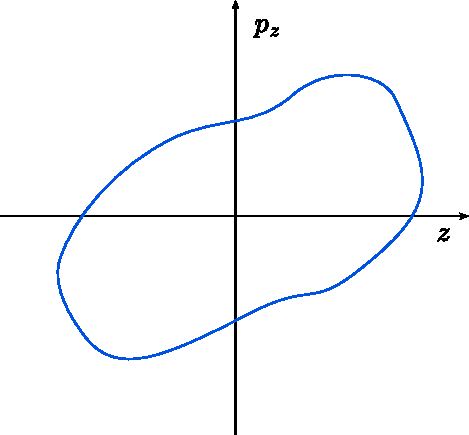
\includegraphics[width=\linewidth]{images/phase_space_regular_coordinates_wonky.pdf}
        %\caption{Caption for Image 1}
        %\label{fig:sub1}
    \end{subfigure}
    \begin{subfigure}[b]{0.292\textwidth}
        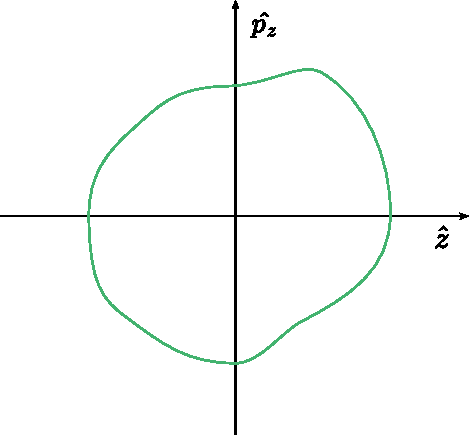
\includegraphics[width=\linewidth]{images/phase_space_normalized_coordinates_wonky.pdf}
    \end{subfigure}
    \begin{subfigure}[b]{0.316\textwidth}
        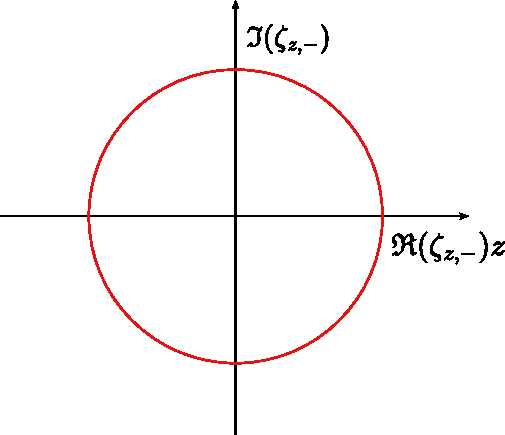
\includegraphics[width=\linewidth]{images/phase_space_normal_form_coordinates.pdf}
    \end{subfigure}
    \caption{Exaggerated phase space distorted by non-linearities described in regular (left),
    normalized (middle) and normal form (right) coordinates.}
    \label{fig:coordinate_systems:distorted_phase_space}
\end{figure}

The map defined previously in \cref{eq:coordinate_systems:non_linear_map} can be rewritten in order
to retrieve an invariant of motion $I_z$ by introducing a generating function $F$:

\begin{equation}
    \tilde{\mathcal{M}} = e^{:-F:} \mathcal{M} e^{:F:}
    \label{eq:coordinate_systems:non_linear_map_normal_form}
\end{equation}



Such a generating function includes all the non-linearities, simplifying the calculations.
Going back and forth from normalized to normal forms coordinates is then straightforward, as
depicted in \cref{fig:coordinate_systems:non_linear_map_normal_form}. The hamiltonian $H$ is now
only dependent on the action $I_z$.


\begin{figure}[H]
    \centering
    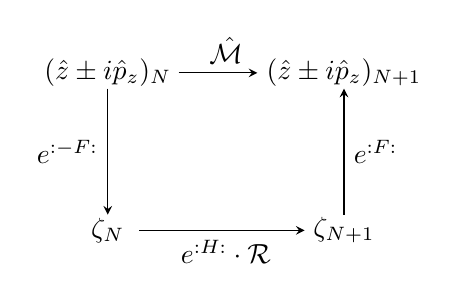
\begin{tikzpicture}[>=stealth]
        % Defining the coordinates
        \coordinate (A) at (0, 0);
        \coordinate (B) at (0, 2);
        \coordinate (C) at (3, 0);
        \coordinate (D) at (3, 2);
        
        % Drawing lines with arrows
        \draw[shorten <=0.2cm, shorten >=0.2cm, ->] (B) -- node[left, text centered] {$e^{:-F:}$} (A);
        \draw[shorten <=0.2cm, shorten >=0.2cm, ->] (C) -- node[right, text centered] {$e^{:F:}$} (D);
        \draw[shorten <=0.4cm, shorten >=0.5cm, ->] (A) -- node[below, text centered] {$e^{:H:} \cdot \mathcal{R}$} (C);
        \draw[shorten <=0.9cm, shorten >=1.1cm, ->] (B) -- node[above, text centered] {$\hat{\mathcal{M}}$} (D);
        
        % Adding labels
        \node at (B) []{$(\hat{z} \pm i\hat{p}_z)_N$};
        \node at (D) []{$(\hat{z} \pm i\hat{p}_z)_{N+1}$};
        \node at (C) [] {$\zeta_{N+1}$};
        \node at (A) [] {$\zeta_{N}$};
    \end{tikzpicture}
    \caption{A one turn map from turn N to N+1 solved using a generating function $F$, 
    transforming to normal form coordinates $\zeta$, applying the linear rotation $R$ and
    transforming back to normalized coordinates.}
    \label{fig:coordinate_systems:non_linear_map_normal_form}
\end{figure}

The function $F$ is defined as

\begin{equation}
    F = \sum_{jklm} f_{jklm}\zeta_{x,+}^j \zeta_{x,-}^k \zeta_{y,+}^l \zeta_{y,-}^m,
\end{equation}

where $f_{jklm}$ are the so-called Resonance Driving Terms (RDTs).  The summation $jklm$ is done
over all the combinations of $j$, $k$, $l$ and $m$ with $j+k+l+m = n$ for a multipole of order $n$,
as shown in \cref{eq:coordinates_systems:sum_jklm},

\begin{equation}
    \sum_{jklm} = \sum_{j=0}^n \sum_{k=0}^n \sum_{l=0}^n \sum_{m=0}^n \quad;\quad j+k+l+m=n.
    \label{eq:coordinates_systems:sum_jklm}
\end{equation}

The expression of the Resonance Driving Terms is given by the global hamiltonian term $h_{jklm}$ by

\begin{equation}
    f_{jklm} = \frac{h_{jklm}}{1 - e^{i2\pi \left[ (j-k)Q_x + (l-m) Q_y \right]}},
    \label{eq:coordinate_systems:fjklm}
\end{equation}

where this coefficient is a summation over the hamiltonian terms of elements $w$ in the lattice,

\begin{equation}
    h_{jklm} = \sum_w h_{w,jklm} e^{i [(j-k)\Delta \phi_x + (l-m) \Delta \phi_y]}.
\end{equation}

The expression of $h_{w,jklm}$ is itself derived from the general hamiltonian 
of \cref{eq:hamiltonian_magnet} by applying a multinomial expansion on the
coordinates~\cite{franchi_studies_2006} as shows \cref{eq:coordinate_systems:hwjklm}.
Derivations and more information on Resonance Driving Terms can be found in \cref{appendix:rdts}.

\begin{equation}
    h_{w,jklm} = -\Re \left[\frac{K_{w,n} + iJ_{w,n}}{j!k!l!m! 2^{j+k+l+m}}
    i^{l+m} \beta_{w,x}^{\frac{j+k}{2}} \beta_{w,y}^{\frac{l+m}{2}} \right]
    \label{eq:coordinate_systems:hwjklm}
\end{equation}

Transforming from the normal form coordinates back to the original normalized coordinates can be
done using the right side of \cref{fig:coordinate_systems:non_linear_map_normal_form}. Which is
written, to second order, as:

\begin{equation}
    \begin{aligned}
        %h_z^{ \pm}
        (\hat{z} \pm i\hat{p}_z) &= e^{: F:} \cdot \zeta_z^{ \pm} \\
                   &\simeq \zeta_z^{ \pm}+\left[F, \zeta_z^{ \pm}\right] 
                        + \frac{1}{2!} \left[ F, \left[ F, \zeta_z^\pm \right]\right].
    \end{aligned}
\end{equation}

Using this equation to the first order and \cref{eq:coordinate_systems:normal_form_coordinates}, the
normalized coordinates can be expressed after $N$ turns in
\cref{eq:coordinate_systems:linear_position_normal_form}.

\small
\begin{equation}
    \begin{aligned}
    (x-ip_x)&(N)= \sqrt{2 I_x} e^{i\left(2 \pi Q_x N+\psi_{x_0}\right)}- \\
    & 2 i \sum_{j k l m} j f_{j k l m}\left(2 I_x\right)^{\frac{j+k-1}{2}}\left(2 I_y\right)^{\frac{l+m}{2}} e^{i\left[(1-j+k)\left(2 \pi Q_x N+\psi_{x_0}\right)+(m-l)\left(2 \pi Q_y N-\psi_{y_0}\right)\right]} \\
    (y-ip_y)&(N)= \sqrt{2 I_y} e^{i\left(2 \pi Q_y N+\psi_{y_0}\right)}- \\
    & 2 i \sum_{j k l m} l f_{j k l m}\left(2 I_x\right)^{\frac{j+k}{2}}\left(2 I_y\right)^{\frac{l+m-1}{2}} e^{i\left[(k-j)\left(2 \pi Q_x N+\psi_{x_0}\right)+(1-l+m)\left(2 \pi Q_y N-\psi_{y_0}\right)\right]} .
    \end{aligned}
    \label{eq:coordinate_systems:linear_position_normal_form}
\end{equation}
\normalsize

This equation highlights the contribution of the non-linear elements to the motion of the particles.
Spectral lines arising from these contributions are discussed in
\cref{section:background:frequency_spectrum}.
It is though to be observed that some $f_{jklm}$ terms will not contribute to the motion in a given
plane due to the dependence on $j$ or $l$.



% ============================================
%           Examples of Maps
% ============================================
\section{\review{Examples of Maps}}
\label{subsection:coordinate_systems:example_of_maps}

It is important to remember that two expansions are used when creating non linear transfer maps.
When referring to the order of a map, it is the order of the BCH formula, used to combine
hamiltonians, that is referred to.
The Lie transformation to transport the coordinates themselves is usually only taken to the first
order.

%----------------------------------------
%         Transfer of 1 Sextupole
%----------------------------------------
\subsection{\review{Non-Linear Transfer of a Single Sextupole}}

Here, we are interested on the effect of a single sextupole on the regular Frenet-Serret coordinates
$x$, $y$, $p_x$ and $p_y$.
Let's consider a sextupole with strength $K_3$ and a normal field,

\begin{equation}
    H_3 = \frac{1}{6} K_3 (x^3 - 3xy^2).
\end{equation}

A transfer map, from longitudinal coordinate $s_0$ to $s_1$, consisting of only this element is the
following:

\begin{equation}
    \begin{pmatrix}
        x \\
        p_x \\
        y \\
        p_y \\
    \end{pmatrix}_{s_1}
    =
    e^{L:H_3:}
    \begin{pmatrix}
        x \\
        p_x \\
        y \\
        p_y \\
    \end{pmatrix}_{s_0},
    \label{eq:coordinate_systems:single_sextupole_lie_transfer}
\end{equation}

where L is the length of the multipole. 
Using \cref{eq:coordinate_systems:expansion_exponential} to expand the Lie transformation to the
first order, it can be rewritten as

\begin{equation}
    \begin{alignedat}{3}
        &e^{L:H_3:} x   &&= x   &&+ [L \cdot H_3, x], \\
        &e^{L:H_3:} p_x &&= p_x &&+ [L \cdot H_3, p_x], \\
        &e^{L:H_3:} y   &&= y   &&+ [L \cdot H_3, y], \\
        &e^{L:H_3:} p_y &&= p_y &&+ [L \cdot H_3, p_y].
        %\numberthis
        \label{eq:coordinate_systems:lie_exponential_first_order_sextupole}
    \end{alignedat}
\end{equation}

Applying the Poisson bracket of \cref{eq:coordinate_systems:poisson_bracket} on $x$ or $y$ yields
$0$, as neither the hamiltonian nor $x$ and $y$ are dependent on $p_x$ and $p_y$,

\begin{equation}
  \begin{aligned}
    [L \cdot H_3, x] &= 
       \overbrace{\frac{\partial (L \cdot H_3)}{\partial x} \frac{\partial x}{\partial p_x}}^{0}
       - \overbrace{\frac{\partial (L \cdot H_3)}{\partial p_x} \frac{\partial x}{\partial x}}^{0}
       + \underbrace{\frac{\partial (L \cdot H_3)}{\partial y} \frac{\partial x}{\partial p_y}}_0
       - \underbrace{\frac{\partial (L \cdot H_3)}{\partial p_y} \frac{\partial x}{\partial y}}_0 \\
                    &= 0.
  \end{aligned}
  \label{eq:coordinate_systems:sextupole_transfer_x_poisson}
\end{equation}


The Poisson bracket applied on $p_x$ or $p_y$ though evaluates to a non-zero value, as the momentum
is present in $p_{x, y}$ while $x, y$ are present in the hamiltonian:

\begin{equation}
  \begin{aligned}
    [L \cdot H_3, p_x] &=
       \frac{\partial (L \cdot H_3)}{\partial x} \frac{\partial p_x}{\partial p_x}
     - \overbrace{\frac{\partial (L \cdot H_3)}{\partial p_x} \frac{\partial p_x}{\partial x}}^{0}
     + \underbrace{\frac{\partial (L \cdot H_3)}{\partial y} \frac{\partial p_x}{\partial p_y}}_0
     - \underbrace{\frac{\partial (L \cdot H_3)}{\partial p_y} \frac{\partial p_x}{\partial y}}_0 \\
                        & = \frac{1}{2} K_3 L (x^2 - y^2)
  \end{aligned}
  \label{eq:coordinate_systems:sextupole_transfer_px_poisson}
\end{equation}

The same method is used for $p_y$.
The final form of the transfer map from \cref{eq:coordinate_systems:single_sextupole_lie_transfer} is
then the following,

\begin{equation}
    \begin{pmatrix}
        x \\
        p_x \\
        y \\
        p_y \\
    \end{pmatrix}_{s_1}
    =
    \begin{pmatrix}
        1 &  &  &  \\
         & 1 + \left(\frac{1}{2 p_x}K_3L(x^2-y^2)\right) &  & \\
         & & 1 & \\
         & &  & 1 - \left(\frac{1}{p_y}K_3Lxy\right)\\ 
    \end{pmatrix}
    \begin{pmatrix}
        x \\
        p_x \\
        y \\
        p_y \\
    \end{pmatrix}_{s_0}.
\end{equation}


It is not necessary to go higher than the first order, as the second order of the expansion of the 
Lie transformation is 0 ; $p_x$ is indeed not present in the result of the first Poisson bracket,

\begin{equation}
    \begin{aligned}
    \frac{1}{2!} [L \cdot H_3, [L \cdot H_3, p_x]]
    &= \frac{1}{2!}\left[L \frac{1}{6} K_3 (x^3 - 3xy^2), \left[L \frac{1}{6} K_3 (x^3 - 3xy^2), p_x\right]\right] \\
    &= \frac{1}{2!}\left[L \frac{1}{6} K_3 (x^3 - 3xy^2), \frac{1}{2} K_3 L (x^2 - y^2)\right] \\
    &= \frac{1}{2!} \cdot 0 \\
    &= 0
    \end{aligned}
\end{equation}



%----------------------------------------
%         Transfer of 2 Sextupoles
%----------------------------------------
\subsection{\review{Non-Linear Transfer of Two Sextupoles}}

It has been seen previously that a single sextupole simply acts as a sextupole when it is alone in the transfer
map, which is expected. Let's now consider two sextupoles which hamiltonians are denoted $H_{1}$ and
$H_{2}$.

Creating a map consisting of only two sextupoles does not make much sense, as it finally results in
one sextupole as their position is the same. Instead, a drift is added between the two elements.
The hamiltonian of a drift of length $L_D$ is given by~\cite{herr_mathematical_2018},

\begin{equation}
    D = -\frac{L_D}{2} (p_x^2 + p_y^2).
\end{equation}

The application of the lie transformation on the canonical coordinates is then very simple, as no
higher orders arise ($[D, [D, x]] = 0$):

\begin{equation}
    \begin{aligned}
        e^{:D:} x   &= x + L_D p_x, \\
        e^{:D:} p_x &= p_x.
    \end{aligned}
\end{equation}

The transfer map of such a line is then the following,

\begin{equation}
    \mathcal{M} = e^{:Z:} = e^{:H_{2}:} \cdot e^{D:H_{1}:},
\end{equation}

describing the evolution of coordinates from a longitudinal position $s_0$ to $s_1$,

\begin{equation}
    \begin{aligned}
        \begin{pmatrix}
            x \\
            p_x \\
            y \\
            p_y \\
        \end{pmatrix}_{s_1}
        =
        \mathcal{M} \cdot
        \begin{pmatrix}
            x \\
            p_x \\
            y \\
            p_y \\
        \end{pmatrix}_{s_0}
    \end{aligned}
    \label{eq:coordinate_systems:transformation_coords_sextupole}
\end{equation}

In order to combine those elements, the BCH formula from \cref{eq:coordinates:bch} is used,
presented here to the third order for two elements,

\small
\begin{equation}
    \begin{aligned}
      Z = \underbrace{H_{2} + H_{1}}_{\text{First order}}
        + \underbrace{\frac{\left[H_{2},H_{1}\right]}{2}}_{\text{Second order}}
        + \underbrace{\frac{\left[H_{2},\left[H_{2},H_{1}\right]\right]}{12} - \frac{\left[H_{1},\left[H_{2},H_{1}\right]\right]}{12}}_{\text{Third order}}
    \end{aligned}
    \label{eq:coordinate_systems:bch_third_order_two_vars}
\end{equation}
\normalsize


\paragraph{First Order}

To the first order, the resulting effective hamiltonian is only the summation of two sextupoles.

\paragraph{Second Order}

The drift added to change the coordinates of $H_1$ allows the Poisson bracket to evaluate to a
non-zero value. Octupolar-like terms indeed appear in the effective hamiltonian. From this, it can
be inferred that two sextupoles will interact together and introduce effects like amplitude
detuning, second order chromaticity and RDTs.
Details of the derivation can be found in~\cref{appendix:transfer_maps}.


\paragraph{Third Order}

To the third order, even higher orders such as decapolar-like effects appear. Such effects
include the third order chromaticity, chromatic amplitude detuning and RDTs.

\paragraph{Remark}

It is to be noted that while sextupoles do introduce higher-order terms, these are often designed to
be small in comparison to those brought by the actual higher-order multipoles, making them thus
often negligible. Such is the case in the LHC.
